\documentclass[9pt, compress]{beamer}
\usepackage{pgfplots}
\usepackage{listings}

\usepackage{tikz, tikz-cd}
\usepackage{amsmath, amsfonts, amsthm, amssymb, mathtools}
\usepackage[all]{xy}
\usepackage{graphicx, wrapfig}
\usepackage{multicol, multirow}
\usepackage{enumerate, enumitem}
\usepackage{esint}
\usepackage[makeroom]{cancel}
\usepackage{upgreek}
\usepackage{xfrac}
\usepackage{makeidx}
\usepackage{marvosym}
\usepackage{ulem}
\usepackage{float}
\usepackage{wasysym}
\usepackage{arydshln}
\usepackage{appendix}
\usepackage{stmaryrd}
\usepackage{mathrsfs}
\usepackage{natbib}
\usepackage{tagging}
\usepackage[brazil, brazilian]{babel}
\usepackage{xalgebra, xtopology, functional} % Pacotes do pablo
\usepackage{hyperref}
\usepackage{fancyvrb}
\usepackage{listings}
\usepackage{centernot}
\usepackage{enumitem}
\usepackage{hyperref}
\usepackage{url}
\usepackage{lipsum}
\usepackage{epigraph}
\usepackage{transparent}
\usepackage[text={}]{draftwatermark}
\usepackage{graphicx}
\usepackage{mathtools}
\usepackage{natbib}
\usepackage{graphicx}
\usepackage{epsfig}
\usepackage{gensymb}
\usepackage{transparent}

% A cor dos link
\definecolor{coolyellow}{RGB}{4, 6, 76}

% Configura a aparência dos link
\hypersetup{
	colorlinks=true,
	citecolor=blue, % Dexa azul po
	linkcolor=coolyellow, 
	%filecolor=magenta,      
	urlcolor=purple,
}

% Configurações gráficas
\usetikzlibrary{calc,shadows.blur}
\pgfplotsset{compat=1.16}

% Corrige o simbolo \qed
\renewcommand{\qedsymbol}{\(\blacksquare\)}

%  Corrige os símbolos de desigualdades
\renewcommand{\leq}{\leqslant}
\renewcommand{\le}{\leqslant}
\renewcommand{\geq}{\geqslant}
\renewcommand{\ge}{\geqslant}
\renewcommand{\preceq}{\preccurlyeq}
\renewcommand{\succeq}{\succcurlyeq}

% Corrige os símbolos de funções
\renewcommand{\to}{\longrightarrow}
\renewcommand{\mapsto}{\longmapsto}

% Conjuntos
\newcommand{\card}[1]{\left\lvert\nobreak#1\nobreak\right\rvert}
\DeclareMathOperator{\ineq}{\underline{\in}}
\DeclareMathOperator{\nieq}{\underline{\ni}}

% Setas que nao vem por padrão
\newcommand{\longhookrightarrow}{\lhook\joinrel\longrightarrow}
\newcommand{\longhookleftarrow}{\longleftarrow\joinrel\rhook}
\DeclareRobustCommand\longtwoheadrightarrow
     {\relbar\joinrel\twoheadrightarrow}

% \sfrac grandao
\newcommand{\mfrac}[2]{{{\Large{\sfrac{{#1}}{{#2}}}}}}


%Símbolos comuns
\DeclareMathOperator{\Mi}{\,\,\geqslant\,\,}
\DeclareMathOperator{\mi}{\,\,\leqslant\,\,}
\DeclareMathOperator{\mif}{\preccurlyeq}
\DeclareMathOperator{\Mif}{\succcurlyeq}
\DeclareMathOperator{\subnvazio}{\underset{^{\neq \varnothing}}{\subset}}
\usepackage{tipa}
\DeclareMathOperator{\vargamma}{\Large\text{\textramshorns}}

%Trigonométricas
\DeclareMathOperator{\sen}{\operatorname{sen}}

% Math symbol font matha
\DeclareFontFamily{U}{matha}{\hyphenchar\font45}
\DeclareFontShape{U}{matha}{m}{n}{
	<5> <6> <7> <8> <9> <10> gen * matha
	<10.95> matha10 <12> <14.4> <17.28> <20.74> <24.88> matha12
}{}
\DeclareSymbolFont{matha}{U}{matha}{m}{n}
\DeclareFontSubstitution{U}{matha}{m}{n}
% Math symbol font mathb
\DeclareFontFamily{U}{mathx}{\hyphenchar\font45}
\DeclareFontShape{U}{mathx}{m}{n}{
	<5> <6> <7> <8> <9> <10>
	<10.95> <12> <14.4> <17.28> <20.74> <24.88>
	mathx10
}{}
\DeclareSymbolFont{mathx}{U}{mathx}{m}{n}
\DeclareFontSubstitution{U}{mathx}{m}{n}

% Symbol definition
\DeclareMathDelimiter{\vvvert}{0}{matha}{"7E}{mathx}{"17}
\newcommand{\trinorma}[1]{\left\vvvert {#1}\right\vvvert}

% Cálculo
\DeclareMathOperator{\del}{\chapterial}
\newcommand{\classe}[1]{\mathscr{C}^{#1}}
\newcommand{\simples}[2]{\displaystyle \dfrac{{\td}{#1}}{{\td}{#2}}}
\newcommand{\parcial}[2]{\displaystyle\dfrac{\partial{#1}}{\partial{#2}}}
\newcommand{\pardois}[3]{\displaystyle\dfrac{\partial^2{#1}}{\partial{#2}\partial{#3}}}
\newcommand{\Lim}[2]{\displaystyle\lim_{#1\to#2}}
\newcommand{\Int}[2]{\displaystyle\int\limits_{#1}^{#2} }
\newcommand{\de}[1]{{\operatorname{d}}{#1}}

% Complexos
\newcommand{\con}[1]{\overline{#1}}
\newcommand{\cis}[1]{\text{cis}\left({#1}\right)}
\newcommand{\ordem}[2]{{\operatorname{ord}}\left({#1},{#2}\right)}
\newcommand{\res}[2]{{\operatorname{Res}}\left({#1},{#2}\right)}

%Abreviações

\newcommand{\evt}{\textsc{evt}}

\newcommand{\vazio}{\varnothing}

\newcommand{\somadir}[3]{
	\underset{{#1}}{\overset{{#2}}{\displaystyle\bigoplus}}\, {#3}
}

\newcommand{\inv}[1]{{#1}^{-1}}

\newcommand{\e}{\hspace{10px}\text{ e } \hspace{10px}}
\newcommand{\tenpx}{\hspace{10px}}

\newcommand{\sigalg}{$\sigma$-álgebra}

% Letras Gregas bbold

\newcommand{\GGamma}{\text{\reflectbox{\rotatebox[origin=c]{180}{$\mathbb L$}}}}
\newcommand{\LLambda}{\text{\reflectbox{\rotatebox[origin=c]{180}{\reflectbox{$\mathbb V$}}}}}
\newcommand{\Eexists}{\text{\reflectbox{$\mathbb E$}}}

\newcommand{\DDelta}{
	\mathrlap{\Delta \hspace{0.105cm}}{
		\begin{tikzpicture}
			\draw (0,0) -- (0,0.000001);
			\draw  (0.0582,0.01 - 0.004) -- 
			(0.0582+0.33*0.31779334981768276,
			0.33*0.6237045669318574- 0.004);
		\end{tikzpicture}\hspace{0.105cm}
	}
}

% Funtores
\usepackage{rotating}
\usepackage{scalerel}

% \covfunctor{F}{A}{B}{X}{Y}{Z}{W}{f}{g}{x}{y} =
% F : A -----→ B
%     X |----→ Y x
%     |        | -
%    f|       g| |
%     ↓        ↓ ↓
%     Z |----→ W y

%This is a first attemp with only 7 arguments
\newcommand{\funtordia}[7]{%
	\begin{tikzcd}[row sep={0.22em}, column sep={0.01em}, ampersand replacement=\&]
		#1: \& {#2} \arrow[rr] \&[1cm]\& {#3} \&   \\
		\& #5 \arrow[d,"#4"'] \arrow[rr, mapsto] \& \& #1(#5) \arrow[d,"#1(#4)"'] \& #7 \arrow[d,mapsto]\\[5mm]
		\& #6 \arrow[rr,mapsto]                     \& \& #1(#6)         \& #7\cdot #4
	\end{tikzcd}
}

%This is taken from the egreg's answer in the link you posted
\ExplSyntaxOn
\NewDocumentCommand{\NewWeirdCommand}{mm}
{% #1 = command to define, #2 = replacement text
	\cs_new:Npn #1 ##1
	{
		\tl_set:Nn \l__covfun_args_tl { ##1 }
		#2
	}
}
\NewDocumentCommand{\Arg}{m}
{
	\tl_item:Nn \l__covfun_args_tl { #1 }
}

\tl_new:N \l__covfun_parse_args_tl
\ExplSyntaxOff


%--------------------------
\NewWeirdCommand{\covfunctor}{%
	\begin{tikzcd}[row sep={0.22em}, column sep={0.01em}, ampersand replacement=\&]
		\Arg{1} \colon \& {\Arg{2}} \arrow[rr] \&[1cm]\& {\Arg{3}} \&   \\
		\& \Arg{4} \arrow[d,"\Arg{8}"'] \arrow[rr, mapsto] \& \& \Arg{5} \arrow[d,"\Arg{9}"'] \& \Arg{10} \arrow[d,mapsto]\\[5mm]
		\& \Arg{6} \arrow[rr,mapsto]                     \& \& \Arg{7}         \& \Arg{11}
	\end{tikzcd}
}
\NewWeirdCommand{\contfunctor}{%
	\begin{tikzcd}[row sep={0.22em}, column sep={0.01em}, ampersand replacement=\&]
		\Arg{1} \colon \& {\Arg{2}} \arrow[rr] \&[1cm]\& {\Arg{3}} \&   \\
		\& \Arg{4} \arrow[d,"\Arg{8}"'] \arrow[rr, mapsto] \& \& \Arg{5} \& \Arg{11} \\[5mm]
		\& \Arg{6} \arrow[rr,mapsto]                     \& \& \Arg{7} \arrow[u,"\Arg{9}"']  \& \Arg{10} \arrow[u,mapsto]
	\end{tikzcd}
}

% Função
\NewWeirdCommand{\function}{%
	\begin{tikzcd}[row sep={0.22em}, column sep={0.01em}, ampersand replacement=\&]
		{\Arg{1}}: \& {\Arg{2}} \arrow[rr] \& [0.5cm] \& {\Arg{3}} \& {\hphantom{\Arg{1}}} \\
		\& {\Arg{4}} \arrow[rr, mapsto] \&  \& {\Arg{5}} \&
	\end{tikzcd}
}


\newcommand{\consep}[1]{{#1}^{\textsc{sep}}}

% Ambientes de teoremas
\newtheorem*{teorema}{Teorema}
\newtheorem*{corolario}{Corolário}
\newtheorem*{lema}{Lema}
\newtheorem*{proposicao}{Proposição}
\theoremstyle{definicao}
\newtheorem*{exemplo}{Exemplo}
\newtheorem*{definicao}{Definição}
\newtheorem*{axioma}{Axioma}
\newtheorem*{invocacao}{Invocação} 
\theoremstyle{remark}
\newtheorem*{afirmacao}{Afirmação} 
\newtheorem*{observacao}{Observação}
\newtheorem*{notacao}{Notação}

% Configura as paradas do Beamer
\usetheme{Rochester}
\usecolortheme{crane}
\usefonttheme{serif}
\setbeamertemplate{itemize items}{\textbullet}
\setbeamertemplate{bibliography item}{\textbullet}

% Configura as bolinha das lista
\setenumerate[0]{label={\color{coolyellow}\normalfont(\roman*)}}
\setitemize{label=\usebeamerfont*{itemize item}%
    \usebeamercolor[fg]{itemize item}
    \usebeamertemplate{itemize item}}

\newcommand{\invlim}{\varprojlim}

\usetag{beamer}

\definecolor{amber}{rgb}{1.0, 0.75, 0.0}
\title{}
\author{}
\date{}

\begin{document}

{\usebackgroundtemplate{%
  \transparent{0.4}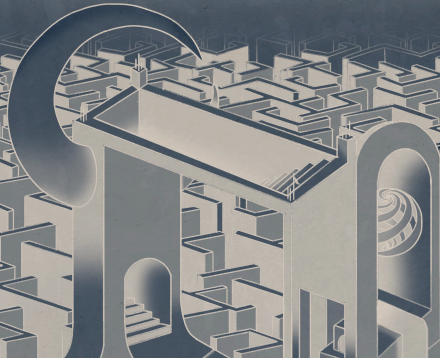
\includegraphics[width=\paperwidth,height=\paperheight]{capa}} 
\begin{frame}
    %\maketitle
\begin{figure}[H]
\centering
    \begin{tikzpicture}{scale=2}
    \node at (0,3) [fill=amber, opacity=0.65] {\huge \begin{tabular}{c}
         \textbf{Operadores de Fredholm entre} \\
         \textbf{\texorpdfstring{\ensuremath{\boldsymbol{C^*}}}{C*}-módulos de Hilbert} 
    \end{tabular}};
    \node at (0,3) {\huge \begin{tabular}{c}
         \textbf{Operadores de Fredholm entre} \\
         \textbf{\texorpdfstring{\ensuremath{\boldsymbol{C^*}}}{C*}-módulos de Hilbert} 
    \end{tabular}};
\node at (0,1) [fill=amber, opacity=0.6] {\Large Gustavo Pauzner Mezzovilla};
\node at (0,1)  {\Large Gustavo Pauzner Mezzovilla};
\end{tikzpicture}
\end{figure}
\end{frame}
\usebackgroundtemplate{}

\section{Pré-requisitos e Motivação}
\begin{frame}{Pré-requisitos}
    \[\boxed{\begin{array}{cl}
       {\footnotesize \textcolor{gray}{1}} & \texttt{\textcolor{red}{import} \textit{C}$^*$-algebras}.\textcolor{blue}{\texttt{complex}} \\
       \pause
       %------------------------------
       {\footnotesize \textcolor{gray}{2}} &\texttt{\textcolor{red}{from} functional-analysis \textcolor{red}{import} hilbert-spaces,} \\
       & \hphantom{\texttt{\textcolor{red}{from} functional-analysis \textcolor{red}{imp}}}\texttt{fredholm-operators}\\ \pause
       %------------------------------

       {\footnotesize \textcolor{gray}{3}} & \texttt{\textcolor{red}{from} ring-theory \textcolor{red}{import} left\_modules,}\\ 
       & \hphantom{\texttt{\textcolor{red}{from} ring-theory \textcolor{red}{impo}}}\texttt{right\_modules, bimodules} \\\pause
       {\footnotesize \textcolor{gray}{4}} & \textcolor{gray}{\texttt{\# \textit{so por seguranca}}} \\
       {\footnotesize \textcolor{gray}{5}} & \texttt{\textcolor{red}{from} \textit{K}-theory.\textcolor{blue}{banach-algebras} \textcolor{red}{import} $K_0, K_1$} \\
        \end{array}}\]
\end{frame}

\begin{frame}[fragile]{Motivação: \textit{Teorema de Exel}}
    \begin{teorema}[Exel (1992)]
        Os $K$-grupos de duas $C^*$-álgebras Morita-Rieffel equivalentes (não necessariamente separáveis) coincidem.
    \end{teorema}

    \textit{Demonstração}. \pause 
    Existe um $(A,B)$-bimodulo $X$ de \textit{imprimitividade} tal que \pause
    $$
    \xymatrix{
    F(A) \ar[r]^{\,\cdot\, \otimes Id_X} \ar[d]_{\operatorname{ind}} & F(B) \ar[d]^{\operatorname{ind}}\\
    K_0(A) \ar@{-->}[r] & K_0(B)
    }$$
    é comutativo.\hfill $\Box$
\end{frame}

\begin{frame}{Hummmm...}
    \begin{figure}[h]
        
\includegraphics[width=0.45\linewidth]{hummm.png}
    \end{figure}
\end{frame}

\begin{frame}{Itinerário}
    \begin{itemize}
        \item Conhecer módulos de Hilbert sobre $C^*$-álgebras.\pause
        \item Conhecer os Operadores de Fredholm entre $C^*$-módulos.\pause
        \item Ter uma noção do \textit{índice} e do isomorfismo $F(A)\longrightarrow K_0(A)$. \pause
        \item Dar um suspiro na motivação do teorema de Exel.
    \end{itemize}
\end{frame}

\section{\texorpdfstring{\ensuremath{C^*}}{C*}-módulos de Hilbert}
\begin{frame}{\texorpdfstring{\ensuremath{C^*}}{C*}-módulos de Hilbert}
\nocite{wegge1993k}
    \begin{definicao}
        Um \textit{$C^*$-módulo de Hilbert} $E$ é um $A$-módulo a direita ($A$ uma $C^*$-álgebra complexa), \pause abençoado com um produto interno\footnote{Linear na 1ª e Involuto-linear; Hermitianidade da Involução e positivo definido.}:
        \begin{equation}
            \langle \,\cdot\,, \,\cdot\,\rangle : E \times E \longrightarrow A
        \end{equation}   
        onde a norma $\Vert x\Vert \coloneqq \sqrt{ \Vert\langle x, x\rangle\Vert}$ é completa.
    \end{definicao}

    \pause

    \begin{observacao}
        \begin{itemize}
            \item \colorbox{red}{\textcolor{white}{\texttt{!Error304 at ``from hilbert-$C^*$-modules import riezs-lemma'' :}}} \colorbox{red}{\textcolor{white}{\texttt{--> \textit{No ``riezs-lemma'' found}}}} \pause 
            \item Nem todo operador linear tem adjunto.
        \end{itemize}
    \end{observacao}
\end{frame}

\section{Operadores Compactos e de Fredholm}

\nocite{gracia2013elements}
\begin{frame}{Digressão: Operadores de Fredholm}
    Os operadores de Fredholm são aqueles $T \in \mathscr B(E,F)$ com núcleo e co-núcleo finito dimensionais, \pause com índice dado
    \[
    \operatorname{ind}(T) \coloneqq \dim \ker T - \dim \ker T^* \in \mathbb Z    
    \]
    \pause
    \begin{invocacao}[Teorema de Atikinson]
        Os operadores de Fredholm são precisamente os invertíveis módulo compacto, \pause i.e., 
        \[
            T :H_1 \longrightarrow H_2 \text{ é Fredholm}\Longleftrightarrow \begin{array}{c}
                \exists\,S: H_2\longrightarrow H_1, \text{t.q.} \\
                Id_{H_2}-ST \text{ e } Id_{H_1}-TS \\
                \text{são compactos}
            \end{array} 
        \]
    \end{invocacao}
\end{frame}

\begin{frame}{\slash\slash\hspace{1cm} entre \texorpdfstring{\ensuremath{C^*}}{C*}-módulos de Hilbert}
    Entre $A$-módulos $E$ e $F$ de Hilbert, operadores da forma $\theta_{x,y} \coloneqq \sum_n y_n \langle x_n, \,\cdot\,\rangle$ são os de \textit{rank-finito}. \pause
    \begin{definicao}[Operadores Compactos]
        $\mathscr K(E,F) \coloneqq \overline{\operatorname{Span}_{x,y} \theta_{x,y}}$ é um ideal bilateral dos adjuntáveis $\mathscr L(E,F)$. 
    \end{definicao}
\pause
    \begin{definicao}
        Os operadores de Fredholm entre $E$ e $F$ são os invertíveis módulo compacto.
    \end{definicao}
\end{frame}

\begin{frame}{Índice}
    Os módulos de \textit{rank-finito} $M$ são os isomorfos a $pA^n$, com $p$ matriz idempotente $n\times n$.\pause
    \[
    \operatorname{rank}(M) \coloneqq [p]_0  \in K_0(A)  
    \]
    \pause
    \begin{proposicao}[Definição do Índice]
         $T:E\longrightarrow F$ é Fredholm $\Leftrightarrow$ são módulos de rank-finito $\ker T$ e $\ker T^*$. \pause O índice de $T$ é dado por
         \[
         \operatorname{ind}(T) \coloneqq \operatorname{rank}(\ker T) -\operatorname{rank}(\ker T^*)   
         \]
    \end{proposicao}
\end{frame}

\section{Um retrato de \texorpdfstring{$K_0(A)$}{K0(A)}}

\begin{frame}{Um retrato de \texorpdfstring{$K_0(A)$}{K0(A)}}
    \begin{teorema}
        É um isomorfismo de grupos 
        $$\operatorname{ind} : \underbrace{\boxed{\,?\,}}_{F(A)} \longrightarrow K_0(A)$$
    \end{teorema}    
\end{frame}

\begin{frame}{Um retrato de \texorpdfstring{$K_0(A)$}{K0(A)}}
    \begin{teorema}
        É um isomorfismo de grupos 
        $$\operatorname{ind} : \underbrace{\dfrac{``{\bigcup\limits_{E,F} \mathscr F(E,F)}"}{\tiny \operatorname{ind}(T_1)=\operatorname{ind}(T_2)}}_{F(A)} \longrightarrow K_0(A)$$
    \end{teorema}    
\end{frame}

\section{Aplicação}

\begin{frame}{Morita-Rieffel}
    \begin{definicao}
        $A$ e $B$ são \textit{Morita-Rieffel} equivalentes $\Leftrightarrow$ existe $X$ um $(A,B)$-bimódulo de imprimitividade: \pause
        \begin{equation*}
        \xymatrix{
         & X \times X \ar[ld]_{(\,\cdot\,\mid\,\cdot\,)} \ar[rd]^{\langle\,\cdot\,,\,\cdot\,\rangle}
         &  \\
        A & & B\\
        }
        \end{equation*}
        \pause
        \begin{itemize}
            \item $\langle X, X\rangle = A$ e $(X\mid X) = B$;\pause
            \item $(x\mid y) z = x \langle y, z\rangle$.
        \end{itemize}
    \end{definicao}\pause
    \textbf{Exemplos}:
    \begin{itemize}
        \item Se $\phi:A\longrightarrow B$ é um isomorfismo, $B$ é um $(A,B)$-bimodulo com $\langle x,y\rangle \coloneqq x^*y$ e $(x,y)\coloneqq \phi^{-1}(xy^*)$. \pause
        \item $H$ espaço de Hilbert e $\mathscr K$ seus operadores compactos. O produto interno
        $$(x,y) \coloneqq \langle\,\cdot\,,y\rangle x$$
        faz com que $H$ seja um $(\mathscr K,\mathbb C)$-bimodulo de imprimitividade.
    \end{itemize}
\end{frame}

\begin{frame}{Isomorfismos estavelmente compactos}
    \begin{teorema}[Brown, Green, Rieffel \cite{brown1977morita}]
        Se $A$ e $B$ são $C^*$-álgebras \underline{separáveis} Morita-Rieffel equivalentes, então
        $$A \otimes \mathscr K \simeq B \otimes \mathscr K$$
        com $\mathscr K\subset \mathscr B(H)$ operadores compactos.
    \end{teorema}
    \pause
    \textit{Be separable, or die!} É uma condição necessária.
    \pause
    \begin{corolario}
        Se $A$ e $B$ são $C^*$-álgebras {separáveis} Morita-Rieffel equivalentes, então
        $$K_0(A) \simeq K_0(B) \text{ e } K_1(A) \simeq K_1(B)$$
    \end{corolario}
\end{frame}

\begin{frame}{Aplicação}
    \begin{teorema}[Exel \cite{exel7fredholm}]
        Se $A$ e $B$ são $C^*$-álgebras \xout{separáveis} Morita-Rieffel equivalentes, o bimódulo de imprimitividade $X$ induz um isomorfismo $X_*$ \pause
        $$
    \xymatrix{
    F(A) \ar[r]^{\,\cdot\, \otimes Id_X} \ar[d]_{\operatorname{ind}} & F(B) \ar[d]^{\operatorname{ind}}\\
    K_0(A) \ar@{-->}[r]_{X_*} & K_0(B)
    }$$
\pause
        Além disso, $SX \coloneqq C_0(\mathbb R) \otimes X$ é um $(SA, SB)$-bimodulo de imprimitividade, e $(SX)_* :K_1(A) \longrightarrow K_1(B)$ também é um isomorfismo.        
    \end{teorema}
\end{frame}

\bibliographystyle{plain}
\bibliography{references}
\end{document}
